% Computational Statistics (Springer Nature) — December 2024 official
% sn-jnl class. Retained historical SMCCA entrypoint: legacy_smcca_main.tex.
% Do not replace this with an unofficial journal class or custom fonts.
\documentclass[pdflatex,sn-mathphys-ay]{sn-jnl}
\usepackage{graphicx}
\usepackage{amsmath,amssymb,amsfonts}
\usepackage{booktabs}
\usepackage{float}
\usepackage{url}
% Original experimental figures are external, publication-sized vector PDFs.
% Springer Nature discourages additional formatting beyond the template.

\newcommand{\R}{\mathbb{R}}
\newcommand{\tr}{\operatorname{tr}}
\newcommand{\diag}{\operatorname{diag}}

\begin{document}

\title[Reusable spectral computation for trend smoothing]{Reusable spectral computation for finite-difference penalized least-squares trends: numerical accuracy and cost}

% Correspondence and affiliation must be verified by both coauthors.
% TODO before submission: add verified \email{...} for corresponding author.
\author*[1]{\fnm{Heriberto} \sur{Espino-Montelongo}}
\author[1]{\fnm{Daniela} \sur{Cort\'es-Toto}}
\affil*[1]{\orgname{Universidad de las Am\'ericas Puebla},
  \orgaddress{\city{San Andr\'es Cholula}, \state{Puebla}, \country{Mexico}}}

\abstract{Finite-difference penalized least squares provides a flexible framework for extracting trends from noisy time series. This study examines a specific computational question: when does reusing a spectral decomposition make smoothing calculations efficient, and how does its numerical behavior compare with structured alternatives? We consider equally spaced observations, a specified difference order, and a fixed mean for the penalized differences. The resulting affine estimator has a polynomial null space and a reusable singular-value representation. This representation permits inexpensive repeated evaluations of effective degrees of freedom and a normalized smoothness index, although reconstructing fitted trends remains more expensive. We also examine the equivalent bounded parameterization of selection criteria through normalized smoothness, including its analytic derivative transformation and inversion costs. We compare fresh and cached dense solvers, a reusable spectral implementation, and a direct banded solver under matched computational workloads, distinguishing preprocessing from repeated evaluations. Deterministic experiments assess numerical agreement and conditioning over several difference orders. A single nonlinear synthetic example illustrates classical smoothing-parameter criteria, and a historical atmospheric carbon-dioxide series illustrates controlled smoothness on observed data. The results characterize workload-dependent computational trade-offs; they do not establish universal speed superiority or forecast accuracy. Joint likelihood estimation of the smoothing parameter and difference mean is outside the scope of this study.}

\keywords{penalized least squares, Whittaker--Henderson smoothing, spectral methods, numerical benchmarking, finite differences}

\maketitle

\section{Introduction}
Finite-difference penalized least squares (PLS) is a well-established approach to extracting a smooth trend from an observed series. Its statistical formulation separates fidelity to the observations from a penalty on successive differences of the trend, as in Whittaker's graduation method and subsequent work \cite{whittaker1923graduation,guerrero2007penalized}. Difference orders beyond two and nonzero reference means are part of this existing family; they are not proposed here as new estimators \cite{guerrero2007penalized,cortes2017smoothness}.

The computational difficulty depends on the task. A single trend at a prescribed penalty can exploit the banded structure of the normal equations, whereas evaluating many smoothing parameters can justify preprocessing a reusable spectral decomposition \cite{weinert2007wh,biessy2026wh}. It is therefore insufficient to compare a cached spectral implementation only with a dense solver that rebuilds the penalty matrix at every step. Likewise, estimating one fitted curve and evaluating a scalar trace-based criterion are different computational workloads.

\emph{Our research question is when reusable spectral computation is competitive for fixed-mean PLS smoothing and how accurately it behaves across difference orders.} We document the affine formulation, effective degrees of freedom, and the option to search an existing criterion over either the penalty or normalized smoothness coordinate; compare four solver strategies under matched workloads; and report deterministic numerical checks, an illustrative synthetic example, and an observed-data smoothing example. We distinguish one-time factorization, repeated complete fits, and repeated scalar trace calculations. This is a bounded computational study of established estimators, not a new smoothing-penalty formulation or a general statistical comparison of selection criteria.

Throughout the computational comparisons, the reference difference mean $\mu$ is fixed numerically, including a prescribed nonzero value in the numerical checks. The library also supports the observed-difference plug-in $\mu=\overline{D_dy}$ and a Gaussian marginal-likelihood selector for fixed or plug-in $\mu$. We retain a short analytical profile-likelihood identity as a pointer to future work, but the present experiments do not validate data-adaptive degrees of freedom, joint $(\lambda,\mu)$ estimation, or a universal ranking of MLE against CV, GCV, AICc, and BIC. Forecast-horizon validation, confidence intervals, and claims of predictive improvement are likewise outside this paper's scope.

\section{Established model and reusable spectral computation}
\subsection{Finite-difference penalized least squares}
Let $y=(y_1,\ldots,y_n)^\top\in\R^n$ denote an equally spaced series. For an integer $1\le d<n$, let $D_d\in\R^{(n-d)\times n}$ represent the $d$th forward-difference operator; for example, row entries of $D_2$ are $(1,-2,1)$. The central estimator is the published penalized least-squares
problem
\begin{equation}\label{eq:objective}
\widehat{\tau}_{\lambda,\mu}
=\arg\min_{\tau\in\R^n}
\left\{
\|y-\tau\|_2^2+
\lambda\|D_d\tau-\mu\mathbf1\|_2^2
\right\},\qquad \lambda\ge0.
\end{equation}
where $\mu\in\R$ is a fixed reference mean for the differences. The choice $\mu=0$ gives the familiar pure penalty. The implementation additionally permits $d=0$, with $D_0=I_n$, as a well-defined edge case; the geometric statements below concern $1\le d<n$.

Write $Q_d=D_d^\top D_d$ and choose $p\in\R^n$ satisfying $D_dp=\mu\mathbf1$. Using zero-based indices $t=0,\ldots,n-1$, one convenient choice is $p_t=\mu\binom{t}{d}$ because $D_d\binom{t}{d}=1$. Setting $x=\tau-p$ and differentiating the strictly convex objective gives
\begin{equation}\label{eq:affine}
 \widehat\tau_{\lambda,\mu}=p+H_\lambda(y-p),\qquad H_\lambda=(I_n+\lambda Q_d)^{-1}.
\end{equation}
Indeed, $(I_n+\lambda Q_d)x=y-p$ and $I_n+\lambda Q_d$ is positive definite for every finite $\lambda\ge0$. This affine expression is equivalent to the normal equations $(I_n+\lambda Q_d)\widehat\tau=y+\lambda\mu D_d^\top\mathbf1$.

\subsection{Proof of the $d$-dimensional kernel}
For $1\le d<n$, the $d$th forward difference has the explicit binomial stencil
\begin{equation}\label{eq:stencil2}
 (D_d\tau)_t=\sum_{k=0}^{d}(-1)^{d-k}\binom{d}{k}\tau_{t+k},\quad
 t=0,\ldots,n-d-1.
\end{equation}
The first $n-d$ columns of $D_d$ form an upper triangular
$(n-d)\times(n-d)$ submatrix with nonzero diagonal $(-1)^d$.
Hence $\mathrm{rank}(D_d)=n-d$. As $Q_d=D_d^\top D_d$,
$x^\top Q_dx=\|D_dx\|^2$, and therefore
\begin{equation}\label{eq:kernel-proof}
\ker Q_d=\ker D_d,\qquad
\dim\ker Q_d=n-\mathrm{rank}(D_d)=d.
\end{equation}
The vectors $1,t,\ldots,t^{d-1}$ have vanishing $d$th forward differences
and are linearly independent on $n>d$ nodes. Thus they give a basis
of the kernel, proving that exactly $d$ eigenvalues of $Q_d$ vanish
in exact arithmetic. Under $\mu=0$, the limit $\lambda\to\infty$
is the least-squares projection onto polynomials of degree $\le d-1$.
For instance $d=1$ preserves a constant, $d=2$ a line, and
$d=3$ a quadratic. When $\mu\ne0$, the limiting set is instead
the affine space $\{\tau:D_d\tau=\mu\mathbf1\}$, which has the same
$d$ homogeneous directions but includes a degree-$d$ particular
solution. In the implementation $p_t=\mu\binom{t}{d}$.

\subsection{Interpretation of higher orders and the spline connection}
For a sufficiently smooth function $f$ observed on an equally spaced
mesh of width $h$, Taylor expansion yields
$\Delta_h^df(x_t)=h^df^{(d)}(x_t)+O(h^{d+1})$. Consequently,
under appropriate mesh-refinement assumptions,
\begin{equation}\label{eq:spline-bridge}
h^{1-2d}\sum_t(\Delta_h^df(x_t))^2
\longrightarrow\int |f^{(d)}(x)|^2\,dx.
\end{equation}
This is a mathematical bridge to roughness penalties in smoothing
splines. A Whittaker-type trend smoother penalizes differences
of fitted ordinates directly, while a $P$-spline instead penalizes
differences of coefficients in a chosen spline basis; these are related
ideas but not identical estimators. For a continuous penalty weight
$\lambda_{\rm cont}$, the corresponding discrete coefficient is scaled
approximately as $\lambda_{\rm disc}=\lambda_{\rm cont}h^{1-2d}$.

The order $d$ is an integer representing the order of the derivative
being approximated; it is not a continuous interpolation between
derivative orders. Comparing different $d$ values is a change of
regularization model, so equal numerical $\lambda$ does not
imply equal smoothing. It is useful to examine orders
$d=1,\ldots,5$ under a common normalized trace-based index;
however, arbitrary orders and polynomial nullspaces have long been
known \cite{weinert2007wh,biessy2026wh}. Larger $d$ can be
ill-conditioned because the binomial stencil has growing coefficients
and the positive eigenvalues may span many orders of magnitude.
Neither higher $d$ nor higher polynomial degree guarantees a better
trend or numerical stability.


\subsection{Null space, SVD, and limiting trends}
The rows of $D_d$ are independent in exact arithmetic, so $\operatorname{rank}(D_d)=n-d$ and $\dim\ker D_d=d$. The null space consists of the sampled polynomials of degree at most $d-1$. Let $D_d=U\Sigma V^\top$ be a full SVD. With nonnegative eigenvalues $\delta_j$ of $Q_d$, ordered so that exactly $d$ are zero, the smoother becomes
\begin{equation}\label{eq:spectrum}
H_\lambda=V\diag\!\left(\frac{1}{1+\lambda\delta_1},\ldots,\frac{1}{1+\lambda\delta_n}\right)V^\top.
\end{equation}
Therefore the transformed observations $c=V^\top(y-p)$ can be computed once, and every new penalty value changes only the scalar attenuation factors $(1+\lambda\delta_j)^{-1}$. At $\lambda=\infty$ the exact limiting fit is $p+P_{\ker D_d}(y-p)$, rather than a computation using an arbitrarily large finite penalty.

For fixed $\mu$, the effective degrees of freedom are $\operatorname{EDF}(\lambda)=\tr(H_\lambda)=\sum_j(1+\lambda\delta_j)^{-1}$. We report Guerrero's trace-based smoothness $S_G=1-\tr(H_\lambda)/n$ alongside the normalized coordinate
\begin{equation}\label{eq:smoothness}
 S(\lambda)=\frac{n-\tr(H_\lambda)}{n-d}\in[0,1],\quad S(0)=0,\quad S(\infty)=1.
\end{equation}
For $1\le d<n$, this coordinate is strictly increasing for finite $\lambda$ because $S'(\lambda)=(n-d)^{-1}\sum_{\delta_j>0}\delta_j/(1+\lambda\delta_j)^2>0$. The normalization changes the scale of the original index but not the ordering of smoothness levels \cite{guerrero2008smoothness}.

\subsection{Interpretation of fixed nonzero differences}
For finite $\lambda$, specifying $\mu\ne0$ shifts the estimator through
the reference vector $p_t=\mu\binom{t}{d}$ in
Eq.~\eqref{eq:affine}; it does not change the smoothing matrix
$H_\lambda$. As $\lambda\to\infty$, the fitted differences satisfy
$D_d\widehat\tau=\mu\mathbf1$, so the limit is a polynomial of
degree at most $d$ rather than at most $d-1$ when $\mu\ne0$.
For example, a prescribed nonzero first-difference mean admits a
linear limiting trend, while a prescribed nonzero second-difference
mean admits a quadratic one. These are known consequences of the
difference penalty and are used here to check implementation
correctness, not to claim a newly introduced family of trends.
All degrees-of-freedom formulas below condition on this fixed
numerical $\mu$.

\subsection{Analytical likelihood profiling: a deferred extension}
For completeness, we retain the key formulas motivating a separate
likelihood-based extension, without incorporating it into the
computational experiments below. Assume a Gaussian model with
independent observation errors of variance $\sigma^2$ and latent
centered $d$th differences of variance $\sigma^2/\lambda$, where
$\lambda>0$. Write $r=n-d$, let $\delta_j>0$ and $v_j$ denote
the $r$ positive-penalty eigenvalues and corresponding eigenvectors
of $Q_d$, and put
\[
p^{(1)}_t=\binom{t}{d},\qquad
z_j=v_j^\top y,\qquad
b_j=v_j^\top p^{(1)},\qquad
w_j(\lambda)=\frac{\lambda\delta_j}{1+\lambda\delta_j}.
\]
Eliminating the unpenalized polynomial coordinates and profiling out
the observation variance gives the marginal negative log-likelihood
criterion, up to constants,
\begin{equation}\label{eq:likelihood-profile}
J(\lambda;\mu)
=r\log\left[\frac1r\sum_{j=1}^r
w_j(\lambda)(z_j-b_j\mu)^2\right]
-\sum_{j=1}^r\log w_j(\lambda).
\end{equation}
For a \emph{fixed positive} $\lambda$, the corresponding optimal
difference mean has the explicit weighted formula
\begin{equation}\label{eq:mu-profile-mle}
\widehat{\mu}(\lambda)=
\frac{\sum_{j=1}^{r}w_j(\lambda)b_jz_j}
{\sum_{j=1}^{r}w_j(\lambda)b_j^2}.
\end{equation}
This reduces the prospective two-parameter optimization to a
one-dimensional profile problem:
\begin{equation}\label{eq:lambda-profile-mle}
\widehat{\lambda}
=\arg\min_{\lambda>0}
J\bigl(\lambda;\widehat{\mu}(\lambda)\bigr).
\end{equation}
These identities are a mathematical outline, \emph{not} a tested
joint-MLE algorithm or a claim of new likelihood theory
\cite{guerrero2007penalized,biessy2026wh}. In particular, the
observed-difference plug-in $\mu=\overline{D_dy}$ is not the
joint likelihood estimate at general positive $\lambda$.
The public implementation currently supports likelihood selection
conditional on a fixed or plug-in $\mu$, not this joint profile.
Identifiability, numerical minimization, inference, and comparative
performance for the joint estimator are left to future work. The
remaining sections evaluate only fixed-$\mu$ smoothing and its
computational costs.

\section{Classical parameter selection and numerical implementation}
\subsection{Selection criteria}
For a fixed numerical value of $\mu$, define $e_\lambda=y-\widehat\tau_{\lambda,\mu}$, $\operatorname{RSS}_\lambda=\|e_\lambda\|_2^2$, $h_{ii}=(H_\lambda)_{ii}$, and $\nu_\lambda=\tr(H_\lambda)$. The classical selectors examined in the single synthetic illustration, following \cite{cortes2017smoothness}, are represented, up to constants irrelevant to an optimizer, by
\begin{align}\label{eq:criteria}
 \mathrm{CV}(\lambda)&=\frac1n\sum_{i=1}^n\left(\frac{e_{\lambda,i}}{1-h_{ii}}\right)^2,\\
 \mathrm{GCV}(\lambda)&=\frac{\mathrm{RSS}_\lambda/n}{(1-\nu_\lambda/n)^2},\\
 \mathrm{AICc}(\lambda)&=\log(\mathrm{RSS}_\lambda/n)+\frac{2\nu_\lambda+1}{n-\nu_\lambda-2},\\
 \mathrm{BIC}(\lambda)&=\log(\mathrm{RSS}_\lambda/n)+\frac{\nu_\lambda\log n}{n}.
\end{align}
The grid-based selection procedure checks denominators, excludes undefined candidates, and compares the exact infinite-penalty candidate. The implementation also supports derivative-based refinement for classical CV and the bounded smoothness search introduced below. In particular, a near-interpolating BIC minimum can be driven by the $\log(\mathrm{RSS})$ boundary, as our example illustrates. We do not interpret a finite-grid BIC minimum close to zero as a universally reliable statistical choice.

Guerrero \cite{guerrero2007penalized} also considers the feasible plug-in $\widehat\mu=\operatorname{mean}(D_dy)$. This option is available \emph{for fitting}; however, the formula for leave-one-out CV in \eqref{eq:criteria} presumes that $\mu$ remains fixed under deletion. The current public selectors intentionally require a fixed numerical $\mu$. Likewise, $\tr(H_\lambda)$ is a conditional EDF and is not automatically the full degrees of freedom of a procedure that estimates $\mu$ from the same observations.

\subsection{Smoothing correction, inversion, and exact endpoints}
With the full orthogonal eigenbasis of the penalty,
$Q_d=V\operatorname{diag}(\delta_1,\ldots,\delta_n)V^\top$,
the $n-d$ positive eigenvalues are $\delta_j=\sigma_j(D_d)^2$,
and the remaining $d$ are zero. Consequently, the spectral
eigenvalues of $H_\lambda=(I+\lambda Q_d)^{-1}$ are
\begin{equation}\label{eq:h-alpha}
\alpha_j(\lambda)=
\begin{cases}(1+\lambda\delta_j)^{-1},&1\le j\le n-d,\\
1,&n-d<j\le n.\end{cases}
\end{equation}
This exposes both the exact limiting polynomial directions and
the scalar attenuation of the penalized directions. If
$\nu(\lambda)=\operatorname{tr}(H_\lambda)
=d+\sum_{j=1}^{n-d}\alpha_j(\lambda)$, the original
trace-based Guerrero index
\begin{equation}\label{eq:original-scale}
S_G(\lambda)=1-\frac{\nu(\lambda)}n
\quad\text{ranges from }0\text{ to }1-\frac dn.
\end{equation}
The upper bound is $1-d/n$, \emph{not} $1-n/d$.
The library also uses a normalized correction:
\begin{equation}\label{eq:normalized-scale}
S(\lambda)=\frac{S_G(\lambda)}{1-d/n}
=\frac{n-\nu(\lambda)}{n-d}\in[0,1].
\end{equation}
The map is strictly increasing for $\lambda\in[0,\infty)$
because
\begin{equation}\label{eq:s-derivative}
S'(\lambda)=\frac{1}{n-d}\sum_{j=1}^{n-d}
\frac{\delta_j}{(1+\lambda\delta_j)^2}>0.
\end{equation}
The exact endpoints are $S(0)=0$ and $S(\infty)=1$;
for any interior target, a one-dimensional bracketed solver
inverts this map. Equal normalized smoothness makes trace scales
comparable across $d$; it does not make the underlying trend
geometries or roughness penalties identical.

\subsection{Where the computational acceleration comes from}
For fixed $\mu$ put $p_t=\mu\binom td$ and
$c=V^\top(y-p)$. One common projection computes $c$; after
that, for each candidate $\lambda$,
\begin{align}\label{eq:fast-profiles}
\operatorname{tr}(H_\lambda)&=d+\sum_{j=1}^{n-d}\alpha_j(\lambda),\\
\|y-\widehat{\tau}_{\lambda,\mu}\|^2
&=\sum_{j=1}^{n-d}(1-\alpha_j(\lambda))^2c_j^2.
\end{align}
Thus a sweep of $M$ values can obtain trace, normalized smoothness,
GCV, AICc, BIC and related scalar profiles in $O(Mn)$
\emph{after} the shared eigendecomposition and $O(n^2)$
projection. A full reconstructed trend remains $O(n^2)$ per
penalty, and exact ordinary CV leverage diagnostics also involve
the spectral basis. The full dense SVD has $O(n^3)$
preprocessing time and $O(n^2)$ storage. This decomposition/reuse
trade-off explains the potential responsiveness of repeated-criteria
explorations without claiming unconditional superiority to
banded linear solvers \cite{weinert2007wh,biessy2026wh}.

Large batches of spectral attenuation operations are naturally
vectorizable. Dense linear algebra can also benefit from optimized
multithreaded BLAS on CPUs. In principle, a GPU backend could
parallelize matrix decompositions and batched matrix operations,
but host/device transfer, synchronization, and initialization
costs may negate a benefit for short series. We found
\texttt{numpy} and \texttt{scipy.linalg.svd} in the package
currently reviewed, not a released GPU solver; therefore no GPU
speedup, power saving, or measured device execution is reported.
A future benchmark should record CPU and GPU models, precision,
BLAS and accelerator versions, transfer time, warmups, memory, and
the number of candidate penalties.


\subsection{Selecting a criterion in normalized smoothness coordinates}
\label{sec:smoothness-coordinate-search}
The monotonicity in Eq.~\eqref{eq:s-derivative} permits a change of
optimization coordinate without changing the underlying PLS estimator
or statistical selection criterion. Write $r=n-d$, let
$\delta_1,\ldots,\delta_r$ denote the strictly positive penalty
eigenvalues, and define
\begin{equation}\label{eq:inverse-s-coordinate}
s=S(\lambda)
=\frac{1}{r}\sum_{j=1}^{r}
\frac{\lambda\delta_j}{1+\lambda\delta_j},
\qquad
\Lambda(s)=S^{-1}(s),\quad 0<s<1.
\end{equation}
Since
\begin{equation}\label{eq:s-coordinate-derivative}
S'(\lambda)=\frac1r\sum_{j=1}^{r}
\frac{\delta_j}{(1+\lambda\delta_j)^2}>0
\qquad (\lambda\ge0),
\end{equation}
$S$ is continuous and strictly increasing, taking the extended
endpoints $S(0)=0$ and $S(\infty)=1$. We define
$\Lambda(0)=0$ and $\Lambda(1)=\infty$ exactly. These formulas
apply for any admissible order $0\le d<n$, provided the positive
penalty spectrum is numerically resolved.

For an existing criterion $C(\lambda;\mu)$ conditional on a fixed
reference mean, introduce $\widetilde C(s;\mu)=C(\Lambda(s);\mu)$.
The same ideal optimization problem can be written as
\begin{equation}\label{eq:criterion-s-coordinate}
\widehat s\in\arg\min_{s\in[0,1]}
\widetilde C(s;\mu),
\qquad
\widehat\lambda=\Lambda(\widehat s).
\end{equation}
Here inadmissible boundary values retain their original definition,
including an undefined ordinary CV score at $\lambda=0$; the
correspondence between global minimizers is set-valued in the
presence of ties. This is an exact reparameterization, not a new
criterion or a proof that a finite numerical search locates the
global optimum. Equal $s$ across difference orders means equal
\emph{normalized conditional trace smoothness}, not equal trend
geometry, variability, or forecast accuracy.

For a differentiable criterion and $0<s<1$, the inverse-function
theorem and the chain rule give
\begin{equation}\label{eq:score-s-chain}
\frac{d\widetilde C}{ds}
=\frac{C'(\lambda)}{S'(\lambda)}
=\frac{dC/d\log\lambda}{dS/d\log\lambda},
\qquad
\frac{dS}{d\log\lambda}
=\frac{1}{r}\sum_{j=1}^{r}
\frac{\lambda\delta_j}{(1+\lambda\delta_j)^2}>0,
\quad\lambda=\Lambda(s).
\end{equation}
Thus interior stationary points coincide in the two
parameterizations. The public implementation exposes the optional
\texttt{search\_space="smoothness"} in
\texttt{select\_lambda}, while
\texttt{search\_space="lambda"} remains the default.
For classical fixed-$\mu$ CV, it scans a uniform and a
logit-spaced set of $s$ values, refines sampled derivative
sign-change brackets and score valleys, and compares evaluated
criterion values at those candidates and exact boundaries.
For GCV, AICc, BIC, and conditional Gaussian MLE the option
evaluates a grid in $s$, using the same score as in $\lambda$.
A user-supplied \texttt{grid} is interpreted in the selected
coordinate. The returned \texttt{lambda\_} remains a penalty;
\texttt{smoothness} returns its normalized trace index,
\texttt{grid} records evaluated penalties, and
\texttt{search\_grid} records the requested coordinates.
Only Gaussian MLE supports the previously defined
observed-difference plug-in for $\mu$; the new coordinate does
not jointly estimate $(\lambda,\mu)$.

The inverse is obtained with a safeguarded root finder in
$\log\lambda$, reusing the spectral representation.
Every interior smoothness evaluation therefore incurs an
additional scalar inversion, typically several $O(r)$
spectral evaluations, before the unchanged criterion score.
Moreover $dS/d\log\lambda$ tends to zero at both limits, so
derivative conversion can be poorly conditioned near $s=0$
or $s=1$. Interior values requiring an unrepresentable
floating-point penalty are rejected rather than silently
treated as endpoints. A bounded search interval does not,
by itself, establish a speed or accuracy advantage over
direct optimization in $\log\lambda$.

For completeness, the prospective joint likelihood profile
in Eq.~\eqref{eq:lambda-profile-mle} could also be expressed
in this coordinate as
\begin{equation}\label{eq:future-joint-s-profile}
\widehat s_{\mathrm{joint}}
=\arg\min_{0<s<1}
J\bigl(\Lambda(s);\widehat\mu(\Lambda(s))\bigr),
\qquad
\widehat\lambda_{\mathrm{joint}}
=\Lambda(\widehat s_{\mathrm{joint}}).
\end{equation}
Equation~\eqref{eq:future-joint-s-profile} describes an
\emph{unimplemented research extension}, not a result of
the conditional-MLE selector or of the benchmarks below.
Boundary candidates and identifiability would require
separate treatment in a full joint-estimation study.


\subsection{Reusable computation and cost}
The reusable \texttt{TrendSmoother(n, order=d)} implementation builds the difference operator and its SVD once. Each candidate $\lambda$ then changes only the spectral attenuation in Eq.~\eqref{eq:spectrum}. The public functions used in this study expose fitted trends, effective degrees of freedom, normalized smoothness, and classical criterion evaluation. The accompanying scripts specify their seeds, inputs, numerical tolerances, and host-recorded timings. The computational experiments, rather than the existence of a Python interface, are the object of evaluation.

The computational trade-off must distinguish decomposition from reuse. A dense full SVD costs $O(n^3)$ preprocessing and $O(n^2)$ memory; after projection, EDF, smoothness, GCV, AICc, and BIC summaries cost $O(n)$ per penalty candidate, while full reconstruction and exact CV leverage scores require $O(n^2)$ each. Smoothness-coordinate selection adds inversion work to each new interior candidate and is therefore not covered by the solver-only timing comparisons. In contrast, the banded structure of $I_n+\lambda Q_d$ allows efficient specialized direct solvers \cite{weinert2007wh}. Thus the phrase \emph{fast computation} means repeated spectral evaluation under a stated workload, not a blanket claim that SVD beats banded factorization. A separate reproducible benchmark in the repository measures setup and fit times independently.

\section{Reproducible numerical illustration}
\subsection{Source-inspired nonlinear design}
To demonstrate the interface without introducing an external data source, we reproduce the nonlinear simulation family of Cort\'es-Toto et al. \cite{cortes2017smoothness}:
\begin{equation}\label{eq:beta}
 \tau(t)=0.6f_{\mathrm{Beta}(30,17)}(t/n)+0.4f_{\mathrm{Beta}(3,11)}(t/n),\quad t=1,\ldots,n.
\end{equation}
We take $n=50$, add independent normal errors with standard deviation $0.5$, omit seasonality, and fix the pseudo-random seed at $19$. These choices define one illustrative replication, not a full reproduction of the article's factorial simulation. We fit $d=2$, $\mu=0$, and select $\lambda$ from the same 121-point geometric grid augmented with the exact $\lambda=\infty$ candidate under each criterion. The latent trend in \eqref{eq:beta} is known, allowing an \emph{ex post} trend-recovery RMSE; it is not a future forecast error.

\begin{figure}[tbp]
\centering
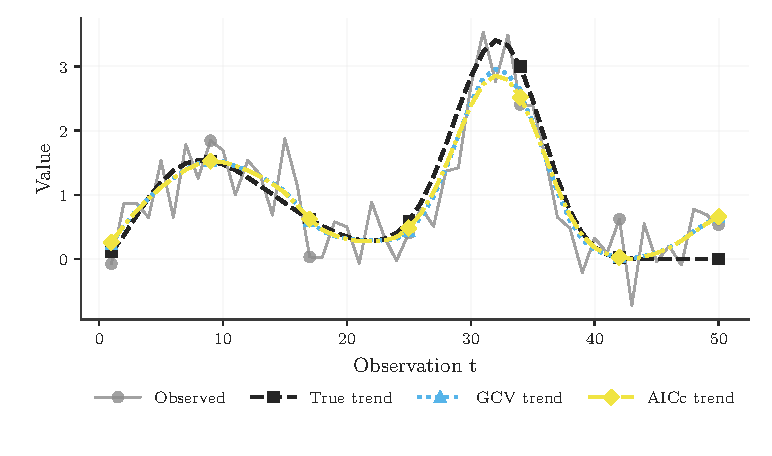
\includegraphics{figures/cortes_toto_synthetic.pdf}
\caption{A synthetic nonlinear case based on Cort\'es-Toto et al. \cite{cortes2017smoothness}. The curves show \emph{in-sample} estimates and known simulated truth, not out-of-sample forecasts. Source data are regenerated by \texttt{figures/make\_figures.py}.}
\label{fig:synthetic}
\end{figure}

\begin{table}[tbp]
\centering
\caption{Selected penalty and normalized smoothness for the case in Fig.~\ref{fig:synthetic}. Trend RMSE is computed against the known latent simulation only.}
\label{tab:criteria}
\input{criteria_table.tex}
\end{table}

As shown in Table~\ref{tab:criteria}, CV and GCV agree in this particular realization, whereas AICc selects a somewhat smoother fit. BIC selects a penalty extremely close to zero on the inspected finite grid; its apparent interpolation tendency illustrates a known practical boundary concern and is not evidence that BIC is generally ineffective. The simulated recoveries are descriptive; no general method ranking follows from a single seed.

\subsection{Algebraic and numerical checks}
An independent check compares the SVD implementation with the direct normal equations for $n=50$, $\lambda=30$, $d\in\{1,2,3\}$ and $\mu\in\{0,0.15\}$ on a second fixed-seed Gaussian sample. The maximum componentwise absolute difference is $2.01\times10^{-12}$ across these six cases, and the limiting constraint $D_d\widehat\tau_{\infty,\mu}=\mu\mathbf1$ holds to maximum error $4.42\times10^{-12}$. Both values result from the supplied deterministic regression script in IEEE double precision; they verify the tested algebra rather than establish stability for all $n,d,\lambda$. In addition, the library regression tests evaluate matched candidate penalties and normalized-smoothness coordinates for $d\in\{0,1,2,4\}$ at a fixed nonzero mean, comparing the original criterion scores after inverse mapping. They also check the smoothness-space CV derivative against centered finite differences. These tests establish numerical agreement at the checked inputs, not faster optimization or identical outcomes of two independently sampled finite grids. Higher differencing orders can be ill-conditioned, and systematic machine-dependent speed measurements remain a distinct stage of the study.

\section{Measured computational cost and repeated parameter evaluation}
\subsection{Experimental design and independent baselines}
Numerical correctness and elapsed time are distinct properties. We
therefore benchmark the same PLS estimator at matched $(n,d,\mu)$
and identical candidate penalties, using four implementations:
(i) a deliberately naive dense solver that reconstructs $D_d$,
$Q_d=D_d^\top D_d$, and solves the normal equations at every
candidate; (ii) a denser but fairer baseline that caches $Q_d$ and
repeats its dense solve; (iii) the reusable full-SVD spectral
implementation of \texttt{TrendSmoother}; and (iv) a banded solver
that assembles $Q_d$ directly in its sparse-band storage and uses
a structure-aware linear solver. The last comparison is crucial:
beating dense normal equations does not imply beating specialized
PLS solvers \cite{weinert2007wh,weinert2012fast}.

\paragraph{Banded factorization and benchmark scope.}
For every finite $\lambda\geq0$, the normal-equation matrix
$A_\lambda=I_n+\lambda D_d^\top D_d$ is symmetric positive
definite, since $x^\top A_\lambda x=\|x\|_2^2+
\lambda\|D_dx\|_2^2>0$ for any nonzero $x$.
It has half-bandwidth $d$, so a banded Cholesky factorization
$A_\lambda=L_\lambda L_\lambda^\top$ is a valid
structure-aware solution method. Its factor generally must be
recomputed when $\lambda$ changes, whereas a spectral basis
can be reused across penalties. This is established computational
prior art \cite{weinert2007wh,weinert2012fast}.

Importantly, the \emph{banded} timings in the four-method
tables below come from \texttt{scipy.linalg.solve\_banded},
a general banded linear-system solver in
\texttt{paper/benchmarks/run\_benchmarks.py}; they are
\emph{not} measured Cholesky timings. The separate library
backend \texttt{PreparedPLSSolver(method="cholesky")} in
\texttt{src/trendestimation/solvers.py} instead calls
\texttt{scipy.linalg.cholesky\_banded} followed by
\texttt{scipy.linalg.cho\_solve\_banded} to produce full
fitted trends. Neither its timings nor Weinert's QR or FFT
methods are included in these four-method tables.
We therefore make no measured Cholesky-specific speed
claim from this experiment.

For every case a deterministic Gaussian sequence is generated,
$\mu$ is held at either zero or a fixed nonzero value, and
$\lambda$ spans $10^{-3}$ to $10^3$ on a geometric grid.
The \texttt{quick} experiment varies $n\in\{40,100,180\}$,
$M\in\{1,16,64\}$ with $d=2$ and adds
$d\in\{1,3,5\}$ at $n=100$, $M=24$, together
with a nonzero-$\mu$ case. The \texttt{full} experiment reaches
$n=400$, $M=256$ and additional difference orders.
All results include one-time setup (not only post-SVD solves);
we record medians, extrema, and median absolute deviations over
repeated independent runs. We bound maximum disagreement against
an independent banded solve for \emph{every} tested penalty.
Runs use a declared random seed, source revision, machine
metadata, NumPy/SciPy versions and a stated BLAS-thread limit.
The code and machine-readable outputs are confined to
\texttt{paper/benchmarks/}.

\begin{table}[tbp]
\centering
\caption{Leading arithmetic complexity for $M$ reconstructed
trends of length $n$ and fixed order $d$. Setup is counted
and no exact operation counts or GPU measurements are asserted.}
\label{tab:complexity}
\begin{tabular}{lll}
\toprule
Method & Setup & Repeated full fits \\
\midrule
Fresh dense solves & rebuilt per $\lambda$ & $O(Mn^3)$ \\
Cached dense $Q_d$ & dense penalty matrix & $O(Mn^3)$ \\
Spectral SVD & $O(n^3)$ & $O(Mn^2)$ \\
Direct banded solver & $O(nd^2)$ & $O(Mnd^2)$ \\
\bottomrule
\end{tabular}
\end{table}

\subsection{End-to-end full-fit timing results}
\IfFileExists{benchmarks/results/full_fit_table.tex}{%
\begin{table}[tbp]
\centering
\caption{Host-measured end-to-end median times in milliseconds, including
one-time setup, for $M$ full fitted trends. Every method computes
the same trends for the same $n$, $d=2$ and $\mu=0$; $R$ is the
naive-fresh-dense time divided by the spectral time. Values and the
numerical parity check are generated from the raw CSV files, not
entered manually.}
\label{tab:full-fit-timings}
\begin{tabular}{rrrrrrr}
\toprule
$n$ & $M$ & Fresh & Cached & Spectral & Banded & $R$ \\
\midrule
40 & 1 & 0.029 & 0.027 & 0.204 & 0.123 & 0.14 \\
40 & 64 & 1.388 & 0.739 & 1.302 & 1.032 & 1.07 \\
100 & 1 & 0.075 & 0.073 & 0.801 & 0.281 & 0.09 \\
100 & 64 & 4.589 & 2.642 & 2.013 & 1.532 & 2.28 \\
200 & 1 & 0.471 & 0.350 & 3.580 & 0.535 & 0.13 \\
200 & 64 & 20.984 & 10.348 & 4.982 & 2.017 & 4.21 \\
400 & 1 & 3.192 & 3.217 & 20.165 & 1.103 & 0.16 \\
400 & 64 & 196.554 & 106.894 & 20.885 & 3.188 & 9.41 \\
\bottomrule
\end{tabular}

\end{table}
}{%
\noindent\emph{No host-verified timing table is bundled:
execute \texttt{python paper/benchmarks/run\_all.py}
on the reference computer to generate the CSV measurements and
LaTeX table before submitting this manuscript.}\par
}
The crossover between methods should be evaluated using
\emph{end-to-end} times, including the SVD setup cost, for both
a single smoothing parameter and a repeated-$\lambda$ sweep.
A ratio greater than one denotes a speed advantage over the
naive baseline on the reported machine, not a universal speedup.
In particular, the structured banded baseline can outperform
a reusable SVD for full trend reconstruction.

\subsection{Scalar smoothness and EDF are different workloads}
To evaluate $\operatorname{tr}(H_\lambda)$ repeatedly, the
spectral method needs only $n-d$ positive eigenvalues:
\[
\operatorname{tr}(H_\lambda)
=d+\sum_{j=1}^{n-d}(1+\lambda\delta_j)^{-1}.
\]
This is $O(Mn)$ work \emph{after} spectral setup, not
$O(Mn^2)$ reconstructed trends. An independent second
experiment compares repeated dense computations
of $\operatorname{tr}[(I+\lambda Q_d)^{-1}]$,
a banded solver applied to all $n$ canonical right-hand
sides, and the spectral sum. The experiment checks
algebraic equivalence separately from timed regions.
Even when the spectral trace is the most efficient
\emph{marginal} score after setup, the $O(n^3)$ SVD cost
can still dominate small workloads.

\IfFileExists{benchmarks/results/trace_table.tex}{%
\begin{table}[tbp]
\centering
\caption{Median end-to-end times (milliseconds) to evaluate $M$
effective-degrees-of-freedom traces, including setup. These entries
measure only scalar $\operatorname{tr}(H_\lambda)$ quantities, not
reconstructed trends.}
\label{tab:trace-timings}
\begin{tabular}{rrrrrr}
\toprule
$n$ & $M$ & Fresh & Cached & Spectral & Banded \\
\midrule
40 & 8 & 0.213 & 0.150 & 0.203 & 0.322 \\
100 & 8 & 1.059 & 0.832 & 0.801 & 1.072 \\
100 & 32 & 4.220 & 3.307 & 0.885 & 3.615 \\
180 & 32 & 15.914 & 12.208 & 2.830 & 10.114 \\
250 & 64 & 92.614 & 59.421 & 6.090 & 38.391 \\
\bottomrule
\end{tabular}

\end{table}
}{}
\IfFileExists{benchmarks/results/benchmark_environment.tex}{%
\noindent\textbf{Measurement provenance:} Platform: Windows-10-10.0.26100-SP0; CPU: Intel64 Family 6 Model 183 Stepping 1, GenuineIntel; Logical CPUs: 32; NumPy: 2.4.6; SciPy: 1.17.1; BLAS threads: 1; Repetitions: 7; Preset: full; Revision: local-unrecorded.

\noindent Maximum observed absolute trend disagreement: $4.32e-10$; maximum EDF trace disagreement: $5.48e-12$.

}{%
\noindent\emph{Computer specifications, software versions, repetition
counts and source revision will appear here after the benchmarks
are run and saved on the reference host.}\par
}

\IfFileExists{figures/full_fit_at_M64.pdf}{%
\begin{figure}[tbp]
\centering
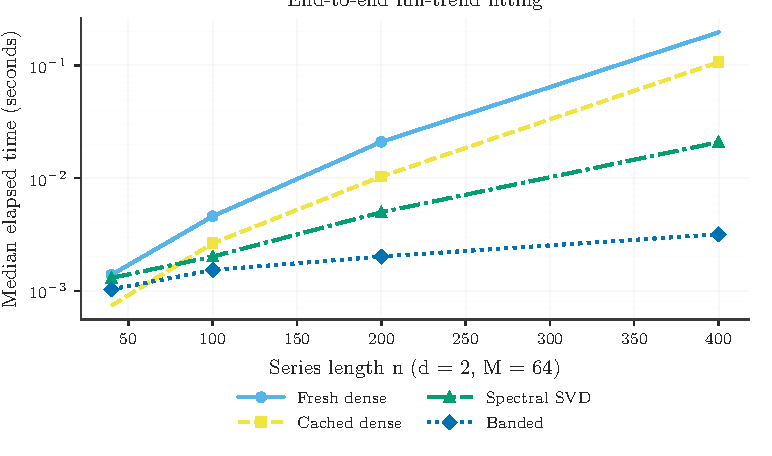
\includegraphics{figures/full_fit_at_M64.pdf}
\caption{End-to-end median times for $M=64$ fitted curves, including setup,
generated on the executing host from the raw CSV files.
These are hardware-specific measurements, not an assumption that
spectral reconstruction is the universally fastest method.}
\label{fig:timing-full}
\end{figure}
}{%
\noindent\emph{The full-fit timing figure is generated after a manually
requested benchmark run with $M=64$.}\par
}

\IfFileExists{figures/trace_at_M32.pdf}{%
\begin{figure}[tbp]
\centering
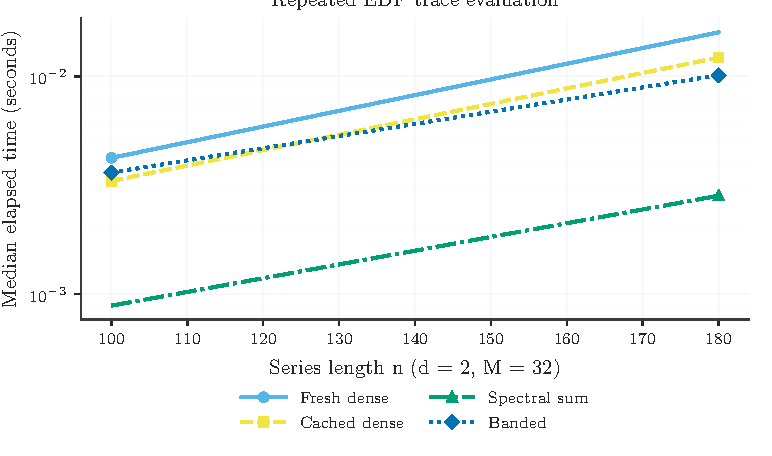
\includegraphics{figures/trace_at_M32.pdf}
\caption{Repeated effective-degrees-of-freedom trace evaluations
($M=32$), including preprocessing. The quantity is scalar
$\operatorname{tr}(H_\lambda)$, not a full trend reconstruction.}
\label{fig:timing-trace}
\end{figure}
}{}

\subsection{Interpreting speed and computational cost}
A timed speed ratio is defined by the two end-to-end
medians, for example
$R_{\rm dense/spectral}
=t_{\rm dense}/t_{\rm spectral}$.
A value above one favors the spectral approach for the
tested workload, not for arbitrary data lengths or
hardware. CPU time, wall time, arithmetic complexity
and energy consumption are different quantities.
CPU numerical libraries already use optimized native
linear algebra, but this experiment does not establish
GPU execution or electricity use. An explicit device
and power measurement would be necessary to make
either claim. Results are intentionally generated
only through a manual command, so the manuscript
does not inadvertently contain timings from a
different machine presented as those of its authors.


\section{A controlled exploration of larger difference orders}
The software accepts any integer $0\le d<n$, but this
algebraic admissibility must be distinguished from
floating-point stability. We therefore conduct a
deterministic diagnostic with $n=50$, seed $24021$,
difference orders $d=1,\ldots,10$, $\mu=0$, and common
normalized smoothness $S=0.86$. At each order,
we form the full SVD of $D_d$, compute the condition ratio
\begin{equation}\label{eq:positive-cond}
\kappa_+(Q_d)=
\frac{\max_{1\le j\le n-d}\delta_j}
{\min_{1\le j\le n-d}\delta_j},
\end{equation}
and compare the spectral fitted trend with an independent
direct solution of $(I+\lambda Q_d)\tau=y$.
The ratio is calculated from the \emph{strictly positive}
penalty eigenvalues; the full $Q_d$ has zero eigenvalues
and is singular for every $d\ge1$.

\begin{figure}[H]
\centering
\begin{tikzpicture}
\begin{axis}[
 width=.92\linewidth,height=5.0cm,
 xlabel={Difference order $d$},
 ylabel={$\kappa_+(Q_d)$},
 ymode=log,
 grid=both,grid style={gray!15},
 xtick={1,2,3,4,5,6,7,8,9,10},
 tick label style={font=\small}]
 \addplot[blue!70!black,thick,mark=*]
 table[x=d,y=condition]{figures/high_order_numerics.dat};
\end{axis}
\end{tikzpicture}
\caption{Condition ratio of the positive spectrum
of $D_d^\top D_d$ for $n=50$, $d=1,\ldots,10$.
Values are recomputed from singular values of $D_d$;
they do not represent hardware-specific runtime.}
\label{fig:high-d}
\end{figure}

The ratio rises from about $10^3$ at $d=1$ to
$2.44\times10^{15}$ at $d=10$.
At $d=10$, the maximum componentwise difference
between the SVD-based fit and the direct normal-equation
solution is approximately $3.36\times10^{-7}$ for the
declared sample and smoothing target, versus
approximately $1.14\times10^{-15}$ at $d=1$.
The direct normal-equation result is not presumed an
exact ground truth at large condition numbers:
both approaches are affected by finite precision.
The experiment illustrates why support for many difference
orders needs accompanying conditioning diagnostics,
rather than establishing new high-order theory,
unconditional stability, or performance superiority.
Machine-specific setup/fitting times are separately
exported by the experiment script for later audit;
they are not promoted to general speed benchmarks.


\section{Observed-data illustration: atmospheric carbon dioxide}
A practical use for trend estimation is the Mauna Loa atmospheric
$\mathrm{CO}_2$ record. These are physical observations, not a
synthetic series. We use the historical weekly concentrations
distributed by \texttt{statsmodels.datasets.co2}
\cite{keeling2004co2,statsmodels2010}, aggregate weekly data
to calendar-month means for 1990--1999, and obtain $n=120$
equally spaced monthly values. No monthly values are missing
within this window. The original monthly sequence mixes an
increasing long-run component with strong seasonal variation;
the latter must not be interpreted solely as instrument noise.

We estimate descriptive low-frequency curves for $d=2,3,4,5$.
Because a conventional GCV grid can select a nearly
interpolating solution in this seasonally varying case,
we instead prescribe the clearly defined normalized
trace-based index $S=0.86$ and solve Eq.~\eqref{eq:normalized-scale}
for $\lambda$ at each order. The resulting penalties are,
respectively, $37.03$, $134.01$, $488.32$, and $1702.30$.
Even at the same normalized $S$, distinct $d$ values
preserve different polynomial directions and may have
different endpoint behavior.

\begin{figure}[tbp]
\centering
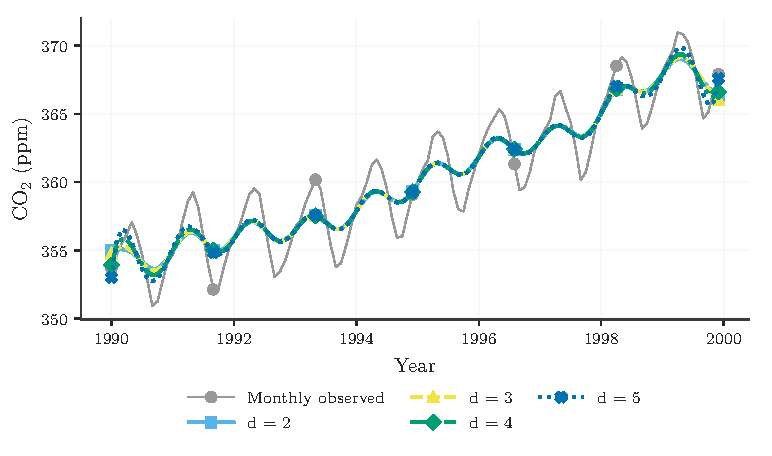
\includegraphics{figures/mauna_loa_1990_1999.pdf}
\caption{Historical Mauna Loa atmospheric carbon dioxide,
monthly aggregates of weekly measurements from 1990--1999,
and two-sided PLS fits with common normalized smoothness
$S=0.86$. These are descriptive trends, not forecasts.}
\label{fig:real-co2}
\end{figure}

The reference mean is fixed at $\mu=0$ for each displayed order,
so the curves show the effect of changing $d$ while keeping the
normalized trace-based smoothness index constant. This descriptive
comparison does not estimate $\mu$ from the data, optimize a Gaussian
marginal likelihood, or provide a forecast evaluation. The observed
seasonal fluctuations should not be interpreted as independent
measurement noise.

A full atmospheric analysis would explicitly model annual
seasonality, measurement uncertainty, and revisions to the
underlying data. The present package smooths the complete
observed series; it does not estimate predictive skill from
future held-out years.


\section{Discussion and conclusions}
For a fixed difference order and reference mean, penalized least-squares
trends can be computed through a reusable spectral representation.
This representation makes repeated scalar trace and smoothness
evaluations inexpensive after decomposition, while reconstructing
complete fitted curves still requires matrix--vector operations.
Our timing experiments compare these tasks separately against fresh
and cached dense solves and a structure-aware banded solver.
The resulting performance comparisons are specific to the reported
data sizes, candidate counts, numerical libraries, and hardware;
in particular, the one-time $O(n^3)$ cost of a full SVD can outweigh
reuse benefits, and banded factorization remains an important
competitor for individual fits.

The deterministic checks support algebraic correctness for the tested
orders and fixed values of $\mu$, while the higher-order diagnostic
also exposes increasing numerical ill-conditioning. The single
nonlinear synthetic example illustrates how established CV, GCV,
AICc, and BIC rules can select different smoothing levels; it is
not a method-ranking experiment. The atmospheric carbon-dioxide
example illustrates historical trend extraction under a specified
normalized smoothness level, not out-of-sample forecast performance.
The normalized coordinate gives a monotone, bounded way to search
existing selection scores while retaining their exact ideal minima.
Its practical appeal is interpretability, but each candidate
requires inverse computation and the chain-rule derivative becomes
sensitive near the endpoints. These additional costs have not
been benchmarked against the log-penalty search in this study.

We therefore delimit the contribution to a reproducible numerical
comparison and implementation analysis of \emph{established}
finite-difference PLS estimators. Estimating $\mu$ jointly with
$\lambda$ by Gaussian marginal likelihood, measuring the statistical
properties of such estimates, and designing forecast-optimal
selection procedures are separate research questions left for
future work. Neither arbitrary difference orders nor nonzero
reference means nor spectral smoothing is claimed to be new.

\section*{Declarations}
% These are editorial placeholders, not statements verified on behalf of the authors.
\noindent\textbf{Funding.} To be confirmed by the authors before submission.

\noindent\textbf{Competing interests.} To be confirmed by the authors before submission.

\noindent\textbf{Ethics approval and consent.} Not applicable to the presented numerical algorithms and historical aggregate time-series examples; authors to verify.

\noindent\textbf{Data availability.} The simulated data can be reproduced from the supplied scripts and seeds. The observed monthly carbon-dioxide series is derived from \texttt{statsmodels.datasets.co2}; data access and provenance are described in the manuscript.

\noindent\textbf{Code availability.} The implementation and paper-specific simulation and benchmark scripts are maintained at \url{https://github.com/heri-espino/trendestimation}. A permanently archived release identifier should be added before submission.

\noindent\textbf{Author contributions.} To be confirmed and approved by both authors before submission.

\bibliography{bibliografia}
\end{document}
